\section{Example Research Applications}
\label{sec:applications}
This section provides a brief overview of research tasks that leverage Project Aria's unique features, from low-level machine perception functions to high-level user- and environment-understanding. Project Aria is designed to enable and connect research across this spectrum: While the former benefits from well-calibrated and understood sensors and access to raw data, the latter can leverage the multiple modalities available or build upon the machine perception functions provided by Aria Machine Perception Services (MPS). 
Note that this is neither an exhaustive review of the respective fields nor a complete list of tasks that are enabled by Project Aria. It is meant to provide examples how Project Aria devices or Aria data can be leveraged, with an emphasis on Aria's unique combination of form-factor, sensors and Machine Perception Services.

\begin{figure}
    \centering
    
{%
\setlength{\fboxsep}{0pt}%
\setlength{\fboxrule}{0.5pt}%
\fbox{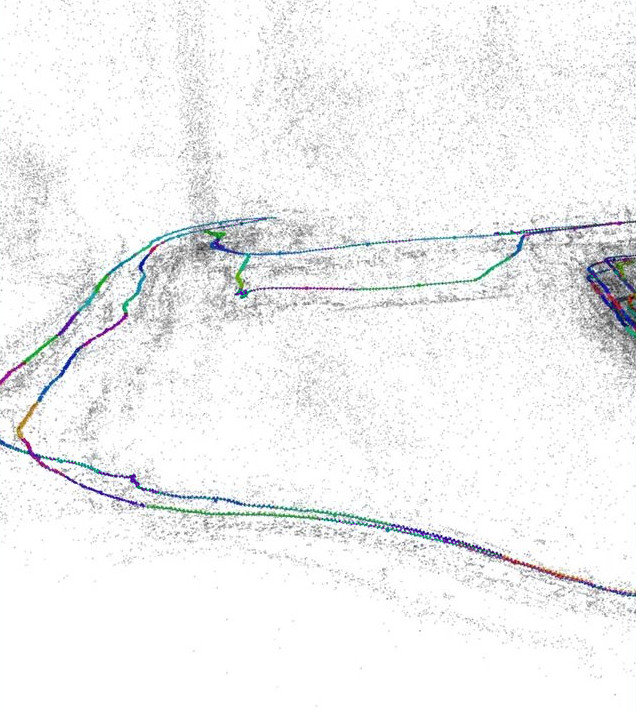
\includegraphics[width=0.325\linewidth]{images/applications/map1.jpg}}\hfill%
\fbox{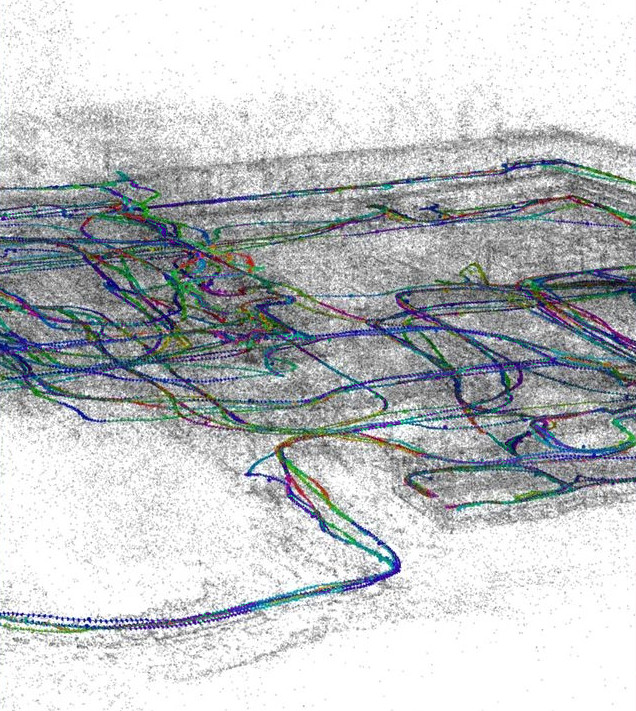
\includegraphics[width=0.325\linewidth]{images/applications/map2.jpg}}\hfill%
\fbox{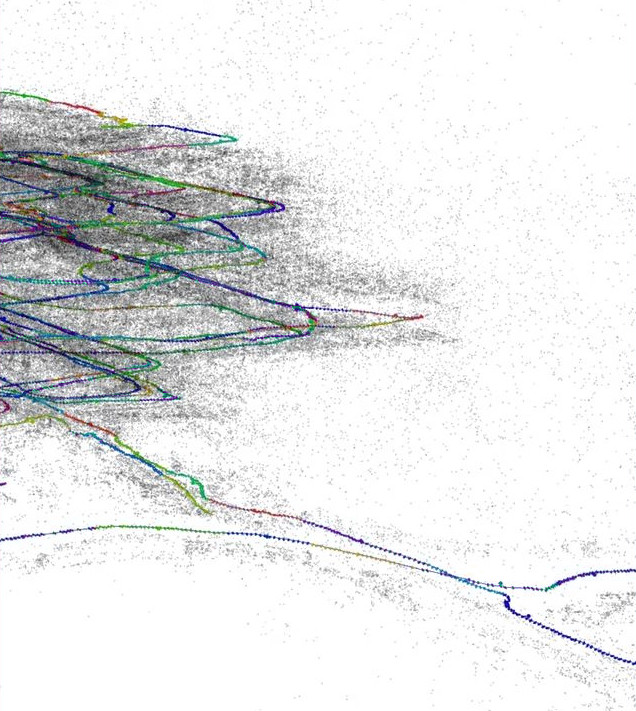
\includegraphics[width=0.325\linewidth]{images/applications/map3.jpg}}%
}
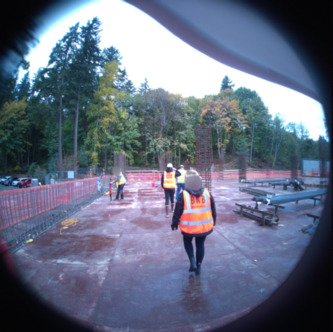
\includegraphics[width=0.16\linewidth]{images/applications/rThumbnail1.jpg}\hspace{0.0065\linewidth}%
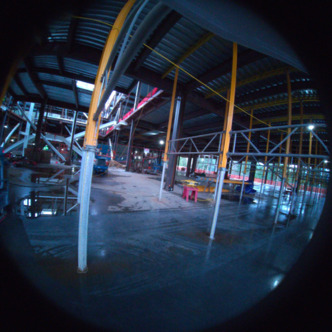
\includegraphics[width=0.16\linewidth]{images/applications/rThumbnail2.jpg}\hspace{0.01\linewidth}%
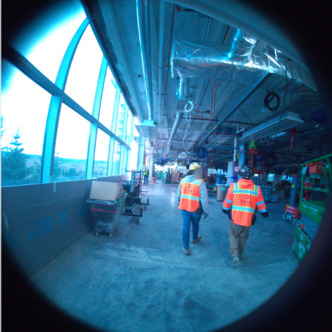
\includegraphics[width=0.16\linewidth]{images/applications/rThumbnail3.jpg}\hspace{0.0065\linewidth}%
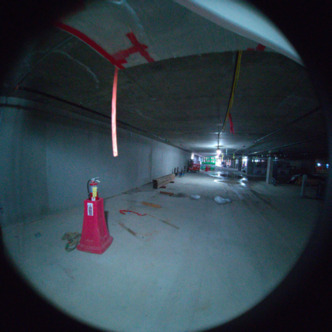
\includegraphics[width=0.16\linewidth]{images/applications/rThumbnail4.jpg}\hspace{0.01\linewidth}%
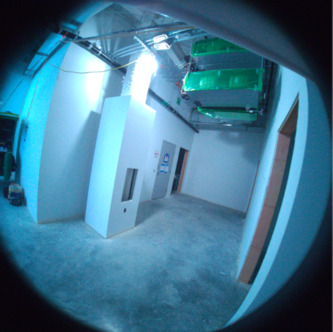
\includegraphics[width=0.16\linewidth]{images/applications/rThumbnail5.jpg}\hspace{0.0065\linewidth}%
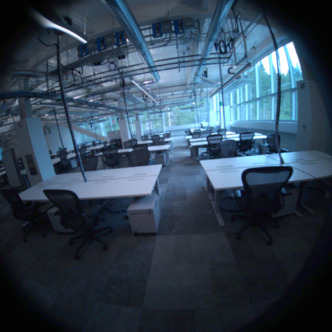
\includegraphics[width=0.16\linewidth]{images/applications/rThumbnail6.jpg}
    \caption{Top: A 3D map created from 275 Aria recordings (175 hours of data), captured over 15 months in a construction site, showing -- from left to right -- the state of the map after one, six, and fifteen months. The images at the bottom are samples from the respective points in time, depicting the transformation from an empty lot to an office building.}
    \label{fig:greenwich}
\end{figure}

\subsection{Life-long Mapping and Re-localization}
Precise 6DoF localization through SLAM or SfM is a common first step across many applications, as well as a base requirement for AR/VR world-locked rendering. It is a comparatively mature field, and Project Aria provides metric 6DoF trajectories as part of Aria MPS (see Sec.~\ref{sec:trajectories}). 
However, many challenges remain: One of these is to reliably re-localize across strong environment changes that occur in natural environments (typically due to lighting, weather, or human activity), as well as updating maps with such changes over time. 
Figure \ref{fig:greenwich} shows a map created from 275 Aria recordings, captured over 15 months, in a building that's being built: Using Aria as convenient recording device and building upon the per-recording trajectories from Aria MPS allows to focus on the core problem of long-range re-localization and map-updating under such strong environmental changes. 



\begin{figure}
    \centering
{%
\setlength{\fboxsep}{0pt}%
\setlength{\fboxrule}{0.5pt}%
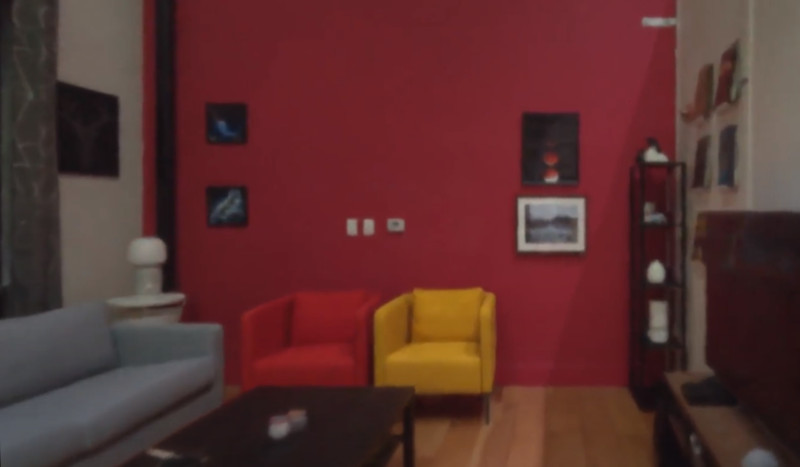
\includegraphics[width=0.495\linewidth]{images/applications/nerf_good.jpg}%
\hfill%
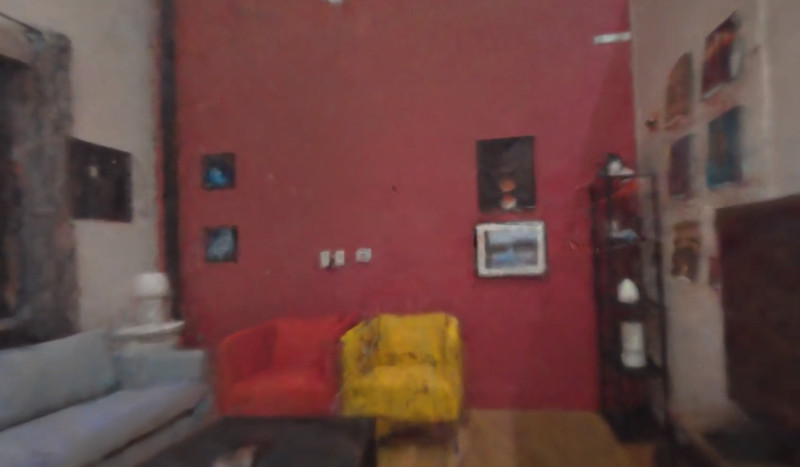
\includegraphics[width=0.495\linewidth]{images/applications/nerf_bad.jpg}\\%
\fbox{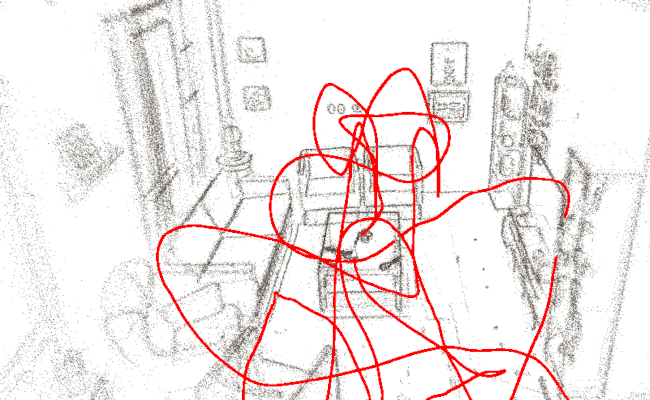
\includegraphics[width=0.49\linewidth]{images/applications/pc_good.png}}%
\hfill%
\fbox{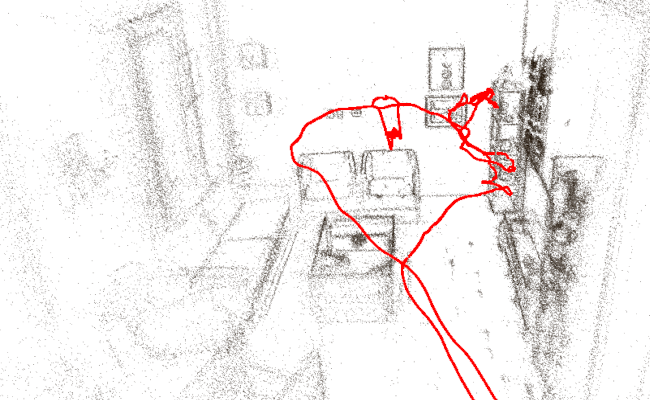
\includegraphics[width=0.49\linewidth]{images/applications/pc_bad.png}}
}%
    \caption{
   Two NeRF reconstructions obtained from Aria recordings using NerfStudio \cite{nerfstudio}. The left shows the result from a carefully curated, hand-held recording that covers the space well and avoids rapid motion. The right shows the result from an egocentric recording during a natural activity. The bottom figures visualize the raw pointcloud and trajectory from MPS. The resulting difference in quality is clearly visible.}
    \label{fig:nerfboxes}
\end{figure}



\subsection{Egocentric Scene Reconstruction and Understanding}
Reconstructing the surrounding scene and semantically identifying objects in it is a key problem for AR/VR applications -- from creating photo-realistic, virtual memories to identifying affordances of objects in the surroundings as part of a context-aware AI assistant. This becomes particularly challenging when the input data is not neatly curated or intentionally taken for this purpose, but rather stems from a form-factor and power-constrained wearable device undergoing natural, unconstrained human motion. 

Figure \ref{fig:nerfboxes} shows the results obtained by state-of-the-art methods for NeRF reconstruction \cite{nerfstudio} on Aria data, comparing careful ``scanning" motion with a natural activity.
 


\subsection{Object Interaction and Manipulation}
Recognizing or tracking objects the user is interacting with, or identifying how the user is interacting with them, is another core egocentric machine perception task. It combines hand-tracking with object tracking, recognition, or scene understanding to connect \textit{things} with user intent or actions. 
Figure \ref{fig:objectinteraction} shows an example application that identifies when the user's hand is near an object in the scene. The approach uses all 3 cameras as well as the trajectory and pointcloud provided by MPS -- which can help in particular to resolve the otherwise common scale/depth ambiguity. Figure \ref{fig:mps_gaze} showed a similar approach using eye gaze to identify what the wearer is looking at. 


\begin{figure}
    \centering
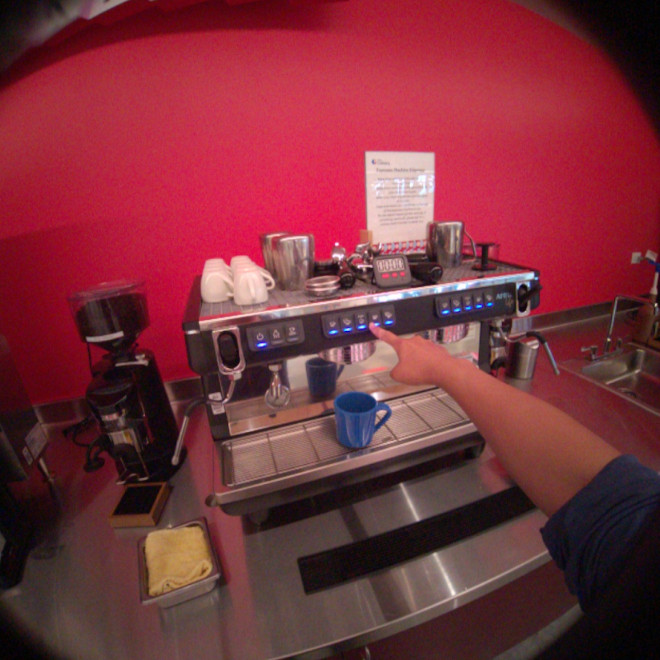
\includegraphics[width=0.49\linewidth]{images/applications/coffee.jpg}%
\hfill%
{%
\setlength{\fboxsep}{0pt}%
\setlength{\fboxrule}{0.5pt}%
\fbox{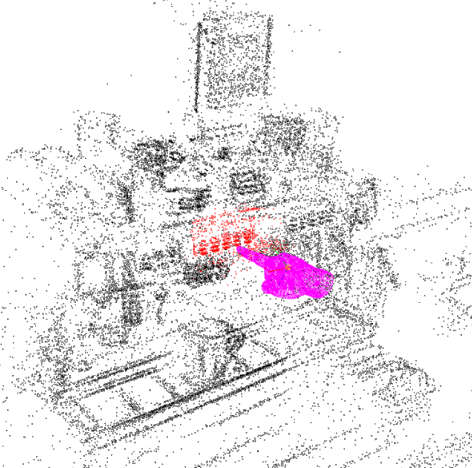
\includegraphics[width=0.49\linewidth]{images/applications/coffee_pc.png}}}
    \caption{We use UmeTrack \cite{han2022umetrack} to track the articulated 3D hand-pose of the wearer in an Aria recording. Combined with the pointcloud from MPS, this allows to identify when the wearer touches a static object. The figures visualize this by coloring points within 8\,cm of the hand in red.}
    \label{fig:objectinteraction}
\end{figure}



%\subsection{Ego-Pose Estimation}
%Of course it's not only the wearer's hands that are relevant: The full, egocentrically estimated body pose is an important input for AR or VR applications, as well as being correlated with the environment, user activity and user intent, making it a valuable signal for contextual AI. 
%Figure X shows an example early result of a full-body pose of the wearer estimated from the 6DoF head-pose, the left and right wrist pose, as well as the pointcloud of the surrounding environment. 


\subsection{Activity Recognition and Attention}
Identifying what the wearer is doing or paying attention to is another likely component of any contextual AI assistant. While much information can be derived from egocentric images or videos alone, significant additional signal can be derived from other modalities, including spatial audio, motion, or eye gaze. 
Figure \ref{fig:activity} shows two example situations where these additional signals allow to disambiguate what the wearer is doing in otherwise ambiguous egocentric views.

\begin{figure}
    \centering
    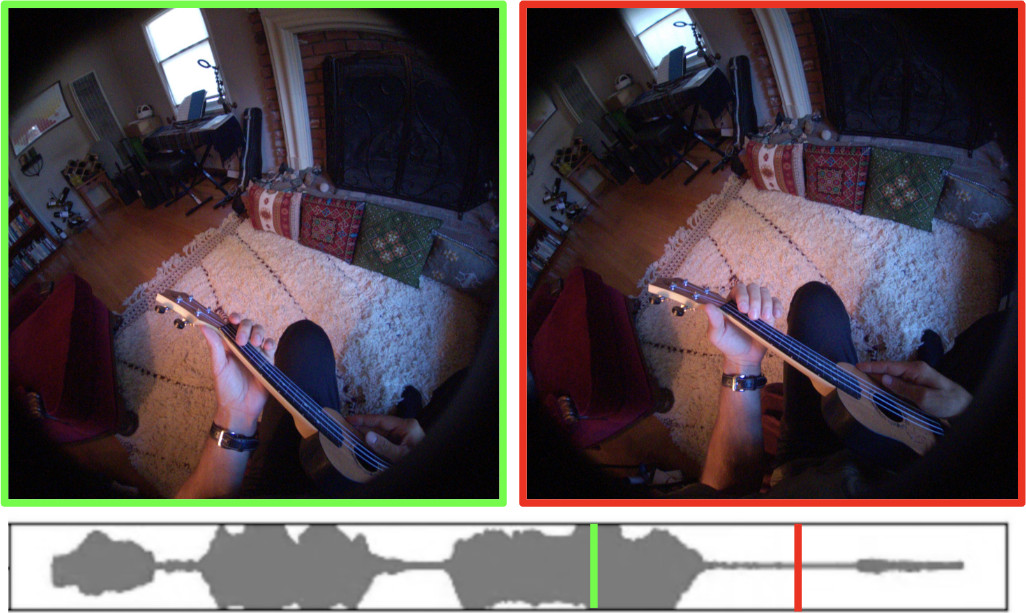
\includegraphics[height=0.37\linewidth]{images/applications/activity_guitar.jpg}\hfill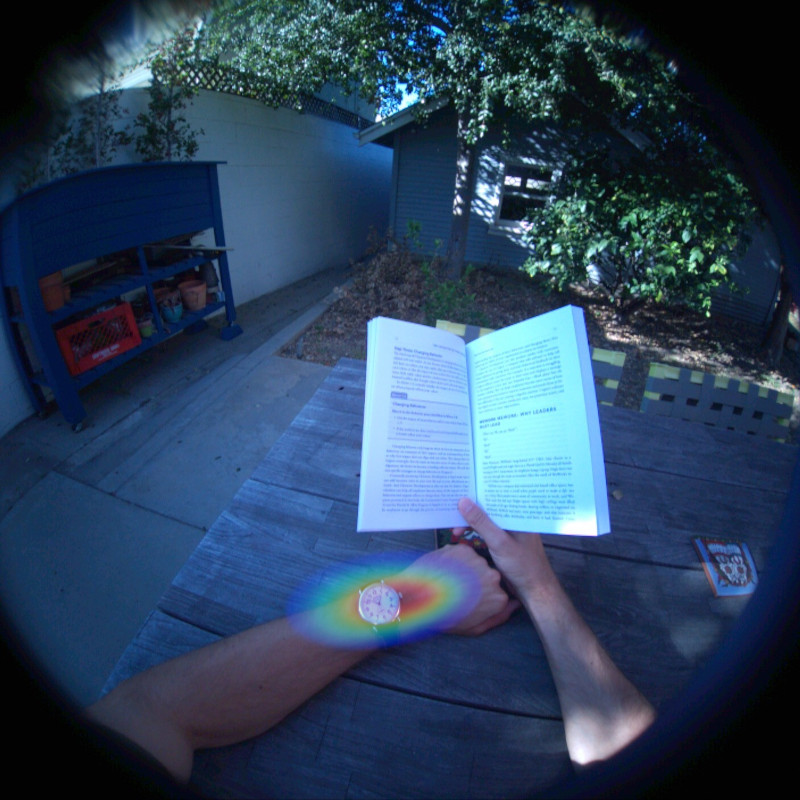
\includegraphics[height=0.37\linewidth]{images/applications/activity_seetime.jpg}
    \caption{Left: two egocentric views of the wearer interacting with a guitar. The audio stream visualized below allows to disambiguate whether the wearer is actively playing or just holding the guitar. Right: the eye gaze (visualized as a heatmap) allows to distinguish whether the wearer is looking at the time or reading a book.}
    \label{fig:activity}
\end{figure}




\subsection{Summarization and Question Answering}
Summarization and Question Answering goes a step further than activity recognition, aiming to summarize relevant events and activities that occur over longer time periods and allowing to answer questions about them. Note that ``relevance" in this context is highly subjective and personal, making signals such as eye gaze or spatial audio key to select the most relevant information for the user. 
%As an example, Figure \ref{fig:summarization} visualizes a situation in which eye gaze and spatial audio are used to estimate which other person the wearer is paying attention to, allowing to isolate and transcribe the relevant portion of the audio signal in a noisy environment.

Furthermore, ``longer time periods" can vary from a few minutes to hours, days, and years -- with longer time-spans becoming increasingly important towards personalized AI assistants, but requiring datasets that do not currently exist. We believe that Project Aria's unique combination of form-factor and machine perception capabilities enables more research in this field towards egocentric, longitudinal summarization and question answering. 

%
%\begin{figure}
%    \centering
%    \begin{minipage}{0.374\linewidth}
%    \includegraphics[width=\linewidth]{images/applications/guitar.jpg}
%    \end{minipage}\hspace{0.025\linewidth}\begin{minipage}{0.6\linewidth}
%    \centering
%    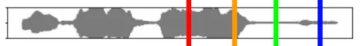
\includegraphics[width=\linewidth]{images/applications/audio.png}\\
%    \textit{\small (transcript of multiple parallel conversations mixed into each other)}\\[-2mm]
%    \rule{\linewidth}{0.2pt}
%    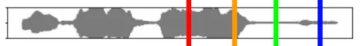
\includegraphics[width=\linewidth]{images/applications/audio.png}\\
%    \textit{\small (transcript of clean conversation from just the one highlighted speaker)}\\
%    \end{minipage}
%    \caption{\textcolor{red}{IMAGES ARE PLACEHOLDERS ONLY} Left: egocentric view in a crowded environment, visualizing also the eye gaze of the wearer that allows to identify whom the wearer is paying attention to. Top-right: environment Audio containing multiple people speaking in parallel. Bottom-right: isolated speech from the speaker the wearer is looking at using [X].}
%    \label{fig:summarization}
%\end{figure}
